\documentclass{article}
\usepackage[T1]{fontenc}
\usepackage[utf8]{inputenc}
\usepackage{lmodern}
\usepackage[ngerman]{babel}
\usepackage{amsmath, amssymb}
\usepackage{array}
\usepackage{phonetic} % for reversed D
\usepackage{wasysym}  % for the notes
\usepackage{tikz, tikzsymbols}
\usepackage{xcolor}
\usetikzlibrary{arrows,automata,fit}
\setlength\parindent{0pt}

    
\begin{document}

\begin{center}
  \Large{Informatik \revD: Übungsblatt 7}

  \large{Sebastian Höffner, Andrea Suckro}
\end{center}



\section*{Aufgabe 7.1}
Gegeben sei: $L=\left\{d^ja^kb^lc^m | (j=0)\text{ oder }(k=l=m) \right\}$

\subsection*{a)}
\subsubsection*{Erste Intuition: Zählvariablen}
Die Sprache beinhaltet die Teilsprache $L_1=\left\{d^ja^kb^lc^m | j>1 \wedge k=l=m \right\}$. Als gute Heuristik zum Abschätzen welcher Sprachklasse eine Sprache angehört, bietet sich an zu untersuchen, wie viele "`Zählvariablen"' abhängig voneinander sind und ob diese beschränkt sind. In der gegebenen Sprache $L_1$ sind drei voneinander abhängige Variablen vorhanden. Ihre Abhängigkeit ist durch $k=l=m$ gegeben. 

Mit regulären Sprachen können wir \emph{keine} Zählvariable "`speichern"' (d.h. \emph{einmal} wiederverwenden), mit kontextfreien \emph{eine} (also zwei Abhängigkeiten zählen). Da wir für diese Sprache drei Zählvariaben haben, können wir zwar gleich viele $b$'s wie $a$'s erzeugen, aber dann keine korrekte Anzahl $c$'s mehr. Die Sprache scheint also intuitiv komplexer als kontextfrei zu sein.

\subsubsection*{Genaueres Hinsehen: Mengeneigenschaften \& Homomorphismus}
Die Sprache $L=\left\{d^ja^kb^lc^m | (j=0)\text{ oder }(k=l=m) \right\}$ besteht aus den Teilmengen $L_l=\left\{d^ja^kb^lc^m | j=0\right\}$ und $L_r=\left\{d^ja^kb^lc^m | k=l=m\right\}$. $L_l$ ist regulär (RegEx: $a^*b^*c^*$). 

$L_r$ ist nicht kontextfrei. Mit Hilfe eines Homomorphismus $h$ ($h(d)=\epsilon, h(a)=a, h(b)=b, h(c)=c$) kann $L_r$ auf $L_r'=\left\{a^ib^ic^i\right\}$ abgebildet werden. Wir wissen, dass diese Sprache nicht kontextfrei ist (siehe Vorlesung Folie 170). Da der Homomorphismus strukturerhaltend ist, ist auch $L_r$ nicht kontextfrei.

Da $L_r \not\subset L_l \wedge L_l \not\subset L_r$ und $L_{l_1} = L_l \setminus \left( L_r \cap L_l \right)$ adjunkt ist zu $L_{r_1} = L_r \setminus \left( L_r \cap L_l \right)$, gibt es Wörter in L, die jeweils nur exklusiv mit $L_l$ oder $L_r$ generiert werden können (für $L_l$ sind das die Wörter $a^kb^lc^m, k\neq l \vee l \neq m \vee m \neq k$, für $L_r$ die Wörter $d^ja^kb^lc^m, j>0 \wedge k=l=m$). Da diese Wörter Teil der Sprache $L$ sind, und die Wörter der Teilmenge $L_{r_1}$ kontextfrei sind, muss intuitiv $L$ ebenfalls kontextfrei sein.


\subsection*{b)}
Wir können nun zwei Fälle betrachten. Erinnerung Regeln für das Pumping Lemma:
\begin{align*}
z &= uvwxy \\
|vx| &\geq 1\\
|vwx| &\leq n \\
\forall i &\geq 0: uv^iwx^iy\in L 
\end{align*}

\subsubsection*{1. Fall $j=0$}
In diesem Fall betrachten wir die Sprache $L'=\left\{a^kb^lc^m\right\} \subseteq L$. Nun versuchen wir darauf das Pumping Lemma anzuwenden. Dazu wählen wir für ein beliebiges Wort $z\in L',|z|\geq n$ (n ist die Mindestwortlänge) folgende Zerlegung: $v\in \left\{a,b,c\right\}$, abhängig davon dass der Buchstabe in dem Wort das wir gerade betrachten vorkommt. $x$ lassen wir komplett leer. Damit ist $|vx| \geq 1$ erfüllt. $w$ können wir ebenfalls leer lassen. Damit ist auch $|vwx| \leq n$ erfüllt. In $u$ und $y$ packen wir die Reste des Wortes. Wenn wir nun $v$ aufpumpen vergrößern wir $k \vee l \vee m$. Für das entstehende Wort gilt weiterhin $uv^iwx^iy \in L'$ und somit auch $uv^iwx^iy \in L$. Das Pumping Lemma ist also für diesen Fall erfüllt.

\subsubsection*{2. Fall $k=l=m$}
In diesem Fall haben wir wieder zwei Fälle. Einmal ist $j=0$, damit landen wir aber im ersten Fall (genauer gesagt ist dann $\left\{a^kb^lc^m|k=l=m\right\} \subset \left\{a^kb^lc^m\right\}$). Im zweiten Fall ist $j>0$. Wir betrachten also $L'=\left\{d^ja^ib^ic^i|j>0\right\}$. Als Zerlegung können wir nun $u$,$x$ und $w$ wieder leer wählen und $v=d^t, t\leq n$ (das bedeutet, dass nicht alle $d$'s in $v$ enthalten sein müssen, da $t\leq j$ sein kann). $|vx| \geq 1$ und $|vwx| \leq n$ sind somit erfüllt. Wenn wir nun $v$ aufpumpen bekommen wir nur $d$'s hinzu und erhalten so wieder ein Wort $z' = uv^iwx^iy \in L'$ und somit auch $z' \in L$.


\section*{Aufgabe 7.2}
Gegeben sei die Sprache $L = \left\{ a^lb^{2^l} \right\}$. Wir nehmen an die Sprache sei kontextfrei. Dann gilt für sie ab einer bestimmten Wortmindestlänge $n$ das Pumping Lemma für Kontextfreie Sprachen. Betrachten wir nun das Wort $a^nb^{2^n}$ Wir überlegen nun welche Buchstaben in $v$ und $x$ sein dürfen, damit das Pumping Lemma überhaupt gelten kann:

\subsection*{Fall 1: $v$ enthält a und b XOR $x$ enthält $a$ und $b$}
Beide Variablen können nicht zugleich $a$'s und $b$'s enthalten, da es nur einen Übergang von $a$ nach $b$ in dem Wort gibt. Sobald $x$ oder $v$ $a$'s und $b$'s enthalten, kann das Aufpumpen nicht mehr funktionieren, da wir dann in das Wort weitere Wechsel von $a$ nach $b$ einbauen, wodurch es nicht mehr $\in L$ ist.

\subsection*{Fall 2: $v$ und $x$ enthalten zusammen nur $a$'s oder nur $b$'s}
$v$ und $x$ können beide komplett in dem $a$- oder $b$-Teil des Wortes liegen. Hier funktioniert jedoch das Aufpumpen ebenfalls nicht, da ich nur eine der beiden Symbole vervielfache und somit wieder das Verhältnis zwischen $a$ und $b$ zerstört wird.

\subsection*{Fall 3: $v$ XOR $x$ sind leer}
Beide Variablen dürfen nicht zugleich leer sein, da sonst die Bedingung $|vx|\geq 1$ verletzt ist. Wenn $x$ oder $v$ leer sind, muss die jeweils nicht leere Variable entweder nur $a$'s oder nur $b$'s enthalten (das entspricht wieder Fall 1). Wenn wir nun aufpumpen zerstören wir damit jedoch aufjedenfall das Verhältnis zwischen $a$'s und $b$'s. Dieser Fall kann also auch keine Worte $\in L$ generieren.

\subsection*{Fall 4: $v$ enthält nur $a$'s und $x$ enthält nur $b$'s}
Dies ist der einzige Fall der uns vielleicht helfen könnte. $v$ enthält in diesem Fall eine bestimmte Anzahl $a$'s und $x$ enthält $b$'s. Natürlich so, dass $|vx| \leq n$ ist. Bei einem beliebigen Aufpumpen bekommen wir nun das Problem, dass die Anzahl der $a$'s linear wächst, während die $b$'s dafür exponential wachsen müsste. Für $i>1$ ist $uv^iwx^iy\in L$ damit nicht mehr erfüllt.

\bigskip

Wir haben für beliebige Worte $\in L$ mit  keine Zerlegung gefunden. Die Sprache $L$ ist folglich nicht kontextfrei.


\section*{Aufgabe 7.3}
\subsection*{Leerheitsproblem}
\begin{center}

\begin{samepage}
Initial:\\
\begin{tabular}{ll}
$S \rightarrow E | ABC$               & $A \rightarrow bDC | E | S$ \\
$B \rightarrow acDC | C$              & $C \rightarrow ab | Ja | IdA$ \\
$D \rightarrow deF | DeF | dEF | DEF$ & $E \rightarrow abba | aBBa | AbbA$ \\
$F \rightarrow JcJ | GJ | bG$         & $G \rightarrow F | IG$ \\
$H \rightarrow SA | Hcc$              & $I \rightarrow c | cIc | dF$
\end{tabular}\\
\end{samepage}

\begin{samepage}
Erster Schritt:\\
\begin{tabular}{ll}
$S \rightarrow {\color{red}E} | AB{\color{red}C}$               & $A \rightarrow bD{\color{red}C} | {\color{red}E} | S$ \\
$B \rightarrow acD{\color{red}C} | {\color{red}C}$              & ${\color{red}C} \rightarrow ab | Ja | {\color{red}I}dA$ \\
$D \rightarrow deF | DeF | d{\color{red}E}F | D{\color{red}E}F$ & ${\color{red}E} \rightarrow abba | aBBa | AbbA$ \\
$F \rightarrow JcJ | GJ | bG$                                   & $G \rightarrow F | {\color{red}I}G$ \\
$H \rightarrow SA | Hcc$                                        & ${\color{red}I} \rightarrow c | c{\color{red}I}c | dF$
\end{tabular}\\
\end{samepage}

\begin{samepage}\clearpage
Zweiter Schritt:\\
\begin{tabular}{ll}
${\color{red}S} \rightarrow {\color{red}E} | {\color{red}ABC}$  & ${\color{red}A} \rightarrow bD{\color{red}C} | {\color{red}E} | {\color{red}S}$ \\
${\color{red}B} \rightarrow acD{\color{red}C} | {\color{red}C}$ & ${\color{red}C} \rightarrow ab | Ja | {\color{red}I}d{\color{red}A}$ \\
$D \rightarrow deF | DeF | d{\color{red}E}F | D{\color{red}E}F$ & ${\color{red}E} \rightarrow abba | a{\color{red}BB}a | {\color{red}A}bb{\color{red}A}$ \\
$F \rightarrow JcJ | GJ | bG$                                   & $G \rightarrow F | {\color{red}I}G$ \\
$H \rightarrow {\color{red}SA} | Hcc$                           & ${\color{red}I} \rightarrow c | c{\color{red}I}c | dF$
\end{tabular}
\end{samepage}
\end{center}
Bereits im zweiten Schritt wird $S$ markiert, also ist $L(G) \neq \emptyset$.

\subsection*{Endlichkeitsproblem}
Wir führen den Algorithmus von oben vorerst zu Ende.
\begin{center}
\begin{samepage}
Dritter Schritt:\\
\begin{tabular}{ll}
${\color{red}S} \rightarrow {\color{red}E} | {\color{red}ABC}$  & ${\color{red}A} \rightarrow bD{\color{red}C} | {\color{red}E} | {\color{red}S}$ \\
${\color{red}B} \rightarrow acD{\color{red}C} | {\color{red}C}$ & ${\color{red}C} \rightarrow ab | Ja | {\color{red}I}d{\color{red}A}$ \\
$D \rightarrow deF | DeF | d{\color{red}E}F | D{\color{red}E}F$ & ${\color{red}E} \rightarrow abba | a{\color{red}BB}a | {\color{red}A}bb{\color{red}A}$ \\
$F \rightarrow JcJ | GJ | bG$                                   & $G \rightarrow F | {\color{red}I}G$ \\
${\color{red}H} \rightarrow {\color{red}SA} | {\color{red}H}cc$ & ${\color{red}I} \rightarrow c | c{\color{red}I}c | dF$
\end{tabular}
\end{samepage}
\end{center}
Weiter lässt sich nichts markieren, d.h. wir können die Grammatik nun auf die markierten Regeln reduzieren.
\begin{center}
\begin{tabular}{ll}
$S \rightarrow E | ABC$            & $A \rightarrow E | S$ \\
$B \rightarrow C$                  & $C \rightarrow ab | IdA$ \\
$E \rightarrow abba | aBBa | AbbA$ & $H \rightarrow SA | Hcc$ \\
$I \rightarrow c | cIc$            & \\
\end{tabular}
\end{center}
Als nächstes reduzieren wir die Grammatik auf erreichbare Regeln.
\begin{center}
\begin{tabular}{ll}
${\color{red}S} \rightarrow {\color{red}E} | {\color{red}ABC}$                         & ${\color{red}A} \rightarrow {\color{red}E} | {\color{red}S}$ \\
${\color{red}B} \rightarrow {\color{red}C}$                                            & ${\color{red}C} \rightarrow ab | {\color{red}I}d{\color{red}A}$ \\
${\color{red}E} \rightarrow abba | a{\color{red}BB}a | {\color{red}A}bb{\color{red}A}$ & $H \rightarrow SA | Hcc$ \\
${\color{red}I} \rightarrow c | c{\color{red}I}c$                                      & \\
\end{tabular}
\end{center}
Übrig bleiben:
\begin{center}
\begin{tabular}{ll}
$S \rightarrow E | ABC$            & $A \rightarrow E | S$ \\
$B \rightarrow C$                  & $C \rightarrow ab | IdA$ \\
$E \rightarrow abba | aBBa | AbbA$ & $I \rightarrow c | cIc$ \\
\end{tabular}
\end{center}
Die Regeln $S \rightarrow E$, $A \rightarrow E$, $A \rightarrow S$ und $B \rightarrow C$ müssen transformiert werden. Die transformierte Grammatik sieht so aus:
\begin{center}
\begin{tabular}{ll}
$S \rightarrow abba | aBBa | AbbA | ABC$ & $A \rightarrow abba | aBBa | AbbA | ABC$ \\
$B \rightarrow ab | IdA$                 & $C \rightarrow ab | IdA$ \\
$E \rightarrow abba | AbbA | aBBa$       & $I \rightarrow c | cIc$ \\
\end{tabular}
\end{center}

Wir erstellen einen Hilfsgraph auf Grundlage der reduzierten und vereinfachten Grammatik.
\begin{center}
\begin{tikzpicture}[->, auto, node distance=2cm]
  \node[state] (S)              {$S$};
  \node[state] (A) [right of=S] {$A$};
  \node[state] (B) [below of=S] {$B$};
  \node[state] (C) [above of=S] {$C$};
  \node[state] (E) [right of=B] {$E$}; 
  \node[state] (I) [left of=S]  {$I$};

  \path (S) edge              node {} (A)
            edge              node {} (B)
            edge              node {} (C)
        (A) edge [bend left]  node {} (B)
            edge [bend left]  node {} (C)
            edge [loop right] node {} (A)
        (B) edge [bend left]  node {} (A)
            edge              node {} (I)
        (C) edge [bend left]  node {} (A)
            edge              node {} (I)
        (E) edge              node {} (A)
            edge              node {} (B)
        (I) edge [loop below] node {} (I)    
        ;
\end{tikzpicture}
\end{center}

Es gibt gerichtete Kreise $B \leftrightarrow A \leftrightarrow C$, sowie $A$ und $I$ auf sich selbst. Somit ist $|L(G)| = \infty$.



\section*{Aufgabe 7.4}
Zur besseren Lesbarkeit wird folgende Bennenung der Elemente der Definition vorgenommen:
\begin{align*}
uUw \rightarrow uyw && U \in V, u,w,y \in \left( V \cup \Sigma \right)^* && |y| \geq 1
\end{align*}

Die Regel $AB\rightarrow BA$ ist nach der neuen Definition nicht erlaubt, da $U \in V$ gegeben ist, somit entweder $A$ oder $B$ der linken Seite das $U \in V$ repräsentiert. Dadurch ergeben sich zwei Fälle:
\begin{itemize}
	\item $U = A$: In diesem Fall wäre auf der linken Seite $w = B$, wodurch aber die Bedingung $uyw$ nicht erfüllt werden kann, da nach $w$ keine Symbole mehr kommen dürfen - in $BA$ wäre das jedoch der Fall.
  \item $U = B$: In diesem Fall ist es umgekehrt: $u = A$, wodurch ebenfalls $uyw$ nicht erfüllt werden kann. Vor $u$ dürfen keine Symbole auftreten, was bei $BA$ jedoch der Fall wäre.
\end{itemize}

\subsection*{Algorithmus}
Um Regeln der Form $VW \rightarrow WV$ ($V, W$ sind Variablen) von der alten in die neue Definition kontext-sensitiver Sprachen zu überführen, geht man wie folgt vor:

\begin{enumerate}
	\item Beginne mit der initialen Definition $VW$, wobei $u=V, U=W, w=\epsilon$. Führe eine neue Variable $X$ ein. Setze $y=X$. Es entsteht die Regel $VW \rightarrow VX$.
  \item Erstelle eine neue Regel $VX \rightarrow WX$ ($u=\epsilon, U=V, w=X, y=W$). 
  \item Erstelle eine weitere Regel $WX \rightarrow WV$ ($u=W, U=X, w=\epsilon, y=V$).
\end{enumerate}
Insgesamt entsteht so ein Regelwerk, dass genau die Regel $AB \rightarrow BA$ in der neuen Definition abbildet.

\subsection*{Konkrekter Fall}
\begin{align*}
\begin{array}{l}
AB \rightarrow AX \\
AX \rightarrow BX \\
BX \rightarrow BA
\end{array}
\end{align*}

\section*{Aufgabe 7.5}
\begin{figure}[!h]
  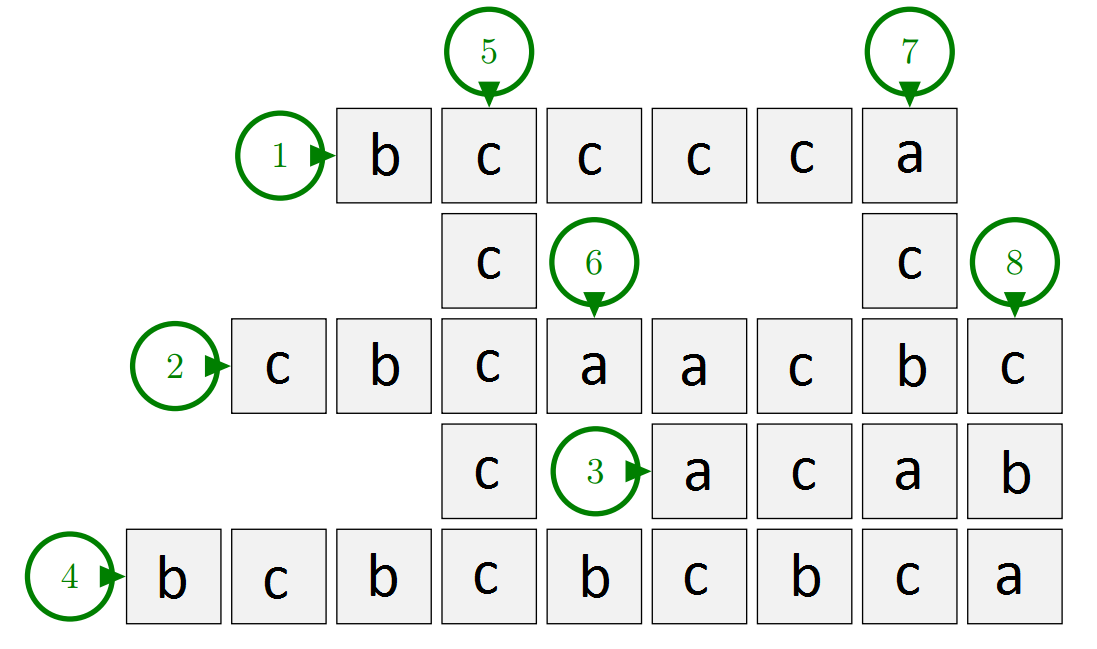
\includegraphics[scale=0.4]{crossword.png}
\end{figure}
\subsection*{Erklärungen}
Die Automaten können etwa in dieser Reihenfolge gut bearbeitet werden:
\begin{enumerate}
	\item[6] Diese Turingmaschine (TM) kann nur $a$ erzeugen, da sie, nimmt man die $b/b,R$ Kante, niemals terminiert.
  
	\item[4] Das zu akzeptierende Wort hat eine ungerade Wortlänge. Dadurch müssen wir die untere $\square/\square,L$ Kante irgendwann erreichen. Dort kann die TM nun deterministisch nur $(bc)^*a$ akzeptieren, das Wort muss also $bcbcbcbca$ sein.
  
	\item[5] Da das letzte Symbol durch 4 mit $c$ gegeben ist, muss vom Start aus die $c/a,R$ Kante genutzt werden, damit durch die $c/a,R$-Schleife dieses $c$ verarbeitet werden kann. Während der ersten Kanten werden so alle Zeichen durch $a$ ersetzt, sogar das erste rechte blank ($\square/a,L$). 
  
  Der nun erreichte Endzustand terminiert aber noch nicht, da durch die Schleife und die Regel $\square/\square,R$ Übergänge möglich sind. Da nun nur $a$'s auf dem Band stehen muss nun der obere Rundgang genutzt werden, der in gleicher Manier alle $a$'s durch $b$'s ersetzt. 
  
  Kommt die TM dann wieder im Startzustand an, ist die Kante $b/\square,R$ nutzbar, die gemeinsam mit der gleich definierten Schleife dafür sorgt, dass die TM mit leerem Band im unteren Endzustand terminiert. Die erste Kante und die darauf folgende Schleife (je $c/a,R$) definieren das akzeptierte Wort: $ccccc$.
  
	\item[7] Diese TM geht ans Ende des Wortes und landet im Endzustand. Dort muss ein $c$ gelesen werden (oder ein $\square$ zum Terminieren gegeben sein), da sonst die TM in den unteren, nicht akzeptierenden Fehlerzustand geht. Nach der gleichen Überlegung muss nun zwingend $a/a,L$, $b/b,L$, $c/c,L$, $a/a,L$, $\square/\square,S$ folgen, das Wort ist also $acbac$.
  
	\item[3] Nach 7 haben wir gegeben, dass das dritte Symbol $a$ sein muss. Die TM hat nur einen möglichen Pfad, der als drittes Zeichen $a$ beinhaltet, wodurch $acab$ als akzeptierendes Wort gefunden werden kann.
  
	\item[8] Die Kante $b/b,S$ führt zu einem Wort $ba(a|b|c)^*$, die Kante $a/b,L$ lässt die TM nicht terminieren und die Kante $c/c,S$ erlaubt Worte der Form $c(a|b|c)^*$. Da der zweite und letzte Buchstabe durch 3 und 4 mit $ba$ gegeben sind, kann das Wort nur $cba$ sein.
  
	\item[2] Diese TM akzeptiert Palindrome. Mit den gegebenen Informationen aus 5, 6, 7 und 8 kann nun einfach der Rest zu $cbcaacbc$ ergänzt werden.
  
	\item[1] Diese TM akzeptiert Wörter, die mit $b$ anfangen, eine gerade Anzahl Symbole haben und an der $n/2+1$-ten Stelle ein $c$ enthält. Die Symbolkette von Stelle 2 bis $n/2$ wir ab Stelle $n/2+2$ wiederholt.
  
  Die erste Hälfte des Wortes wird nach und nach (beginnend rechts) durch $\$$ ersetzt, die zweite (ebenfalls von rechts) einfach gelöscht ($\square$). Am Ende werden die $\$$ ebenfalls durch $\square$ ersetzt und das Wort akzeptiert.
  
  
  Da bereits an zweiter Stelle $c$ und an letzter Stelle $a$ gegeben sind, das Wort mit b beginnen muss und an der $n/2+1$-ten Stelle das $c$ durch das b gegeben ist, bleibt nur noch die Möglichkeit $bcacca$.
\end{enumerate}


\section*{Aufgabe 7.6}
\begin{center}
\textbf{Vom süßen Brei (1815)}

\textit{\footnotesize{aus: Brüder Grimm. Kinder- und Haus-Märchen Band 2, Große Ausgabe.}}
\end{center}
\begin{flushleft}\small
Es war einmal ein armes, frommes Mädchen, das lebte mit seiner Mutter allein und sie hatten nichts mehr zu essen. Da ging das Kind hinaus in den Wald und begegnete ihm darin eine alte Frau, die wußte seinen Jammer schon und schenkte ihm ein Töpfchen, zu dem sollt' es sagen: "`Töpfchen koch!"' so kochte es guten, süßen Hirschenbrei, und wenn es sagte: "`Töpfchen steh,"' so hörte es wieder auf zu kochen. Das Mädchen brachte den Topf seiner Mutter heim und nun waren sie ihrer Armuth und ihres Hungers ledig und aßen süßen Brei, so oft sie wollten. Auf eine Zeit war das Mädchen ausgegangen, da sprach die Mutter: "`Töpfchen koch!"' da kocht es und sie ißt sich satt; nun will sie, daß das Töpfchen wieder aufhören soll, aber sie weiß das Wort nicht. Also kocht es fort und der Brei steigt über den Rand heraus, und kocht immer zu, die Küche und das ganze Haus voll, und das zweite Haus und dann die Straße, als wollt’s die ganze Welt satt machen, und ist die größte Noth und kein Mensch weiß sich da zu helfen. Endlich, wie nur noch ein einziges Haus übrig ist, da kommt das Kind heim und spricht nur: "`Töpfchen steh!"' da steht es und hört auf zu kochen, und wenn sie wieder in die Stadt wollten, haben sie sich durchessen müssen.
\end{flushleft}

\subsection*{Inhalt}
Der Inhalt ist somit geklärt: Ein Mädchen bekommt einen kleinen Topf, dieser kocht für sie unendlich viel Brei bis sie ihn stoppt. Das führt natürlich zur Katastrophe, der mit Brei gefüllten Stadt. Die Katastrophe wird jedoch humorvoll gelöst: Das Töpfchen wird gestoppt und es passiert nichts weiter Schlimmes, als dass nun die Bewohner der Stadt sich durch den Brei essen müssen, um zurück zu ihren Häusern zu gelangen.

\subsection*{Beziehung Märchen - Erfindung}
Die Beziehung zwischen Märchen und der "`sehr vertrauten "`Erfindung"' von Stephen Cole Kleene"' ist ebenfalls simpel: 
Der Kleene-Stern funktioniert ein wenig wie das Töpfchen. Das Töpfchen produziert immer weiter Brei, während der Stern immer weiter Zeichen akzeptiert bzw. generiert (je nach Anwendungs- bzw. Interpretationskontext). 

\subsection*{Rolle von Kleene}
Die Frage, welche Rolle Kleene in diesem Märchen einnehmen würde, ist etwas komplizierter zu klären. In dem Märchen gibt es prinzipiell vier Rollen: Das Mädchen, die Mutter, die alte Frau und das Töpfchen. 
\begin{itemize}
	\item Da wir bereits klärten, dass das Töpfchen dem Kleene-Stern entspricht, liegen zwei Personen für Kleene nahe: Das Mädchen oder die alte Frau. Die Mutter ist auszuschließen, da diese die Katastrophe herbeiführt - Kleenes Erfindung ist aber eher nütz- als hinderlich.
  \item Die alte Frau hat das Töpfchen zuerst und gibt es dem Mädchen. Sie stellt viele Fragen: Woher ist das Töpfchen, warum ist sie im Wald, ...? Die Antwort ist: Die alte Frau steht für etwas, das vor dem Mädchen (und vielleicht dem Töpfchen?) existierte. Im übertragenen Sinne können wir sie als Symbol für die Mathematik, die Informatik oder auch ganz konkret die Automatentheorie oder Rekursionstheorie sehen. 
  \item Das Mädchen bekommt das Töpfchen von der alten Frau. Es also ein Werkzeug, um ein Problem zu lösen (in der Geschichte der Hunger und die Armut). Dieses Werkzeug macht sie sich zu nutzen und stellt es auch anderen zu Verfügung, die jedoch erst lernen müssen, es zu verwenden. 
\end{itemize}

Kleene handelt wie das Mädchen: Er erhält bzw. erfindet ein Werkzeug um ein Problem zu lösen. Das Werkzeug ist der Kleene-Stern, bzw. die mathematische Idee, die er repräsentiert. Kleene bekommt die Idee aus der Mathematik, indem er versucht das Problem zu lösen, Schleifen in Automaten sinnvoll beschreiben zu können. Wie das Mädchen, das in den Wald ging, um den Hunger zu stillen, sucht Kleene in der Mathematik nach dieser Lösung und bekommt sie. Wie das Mädchen bringt er das Werkzeug zu anderen, die es ebenfalls gern nutzen möchten - den Umgang aber erst lernen müssen. Kleenes Rolle wäre somit klar die des Mädchens.



\end{document}
